\documentclass{beamer}
\usepackage[T1]{fontenc}
\usepackage[polish]{babel}
\usepackage[utf8]{inputenc}
\usepackage{graphicx}
\usepackage{listings}

\definecolor{custom blue}{RGB}{51, 77, 204}

\usetheme{CambridgeUS}
\usecolortheme{whale}
\setbeamercolor{frametitle}{bg=custom blue, fg=white}
%\setbeamercolor{title}{bg=deep sky blue, fg=black}

\graphicspath{ {./assets/} }
\setbeamertemplate{footline}{
    \hfill\insertframenumber/\inserttotalframenumber\hspace{1em}
}

\title{Komunikacja międzyprocesowa z D-Busem} 
\author{Maksymilian Wnuk}  
\date{\today} 

\begin{document}

\begin{frame}
    \titlepage
\end{frame} 

\begin{frame}
\frametitle{Plan}
\begin{itemize}
    \item Historia
    \item Teoria
    \item Praktyka
\end{itemize}
\end{frame}

\section{Historia}


\begin{frame}
\frametitle{Komunikacja międzyprocesowa}
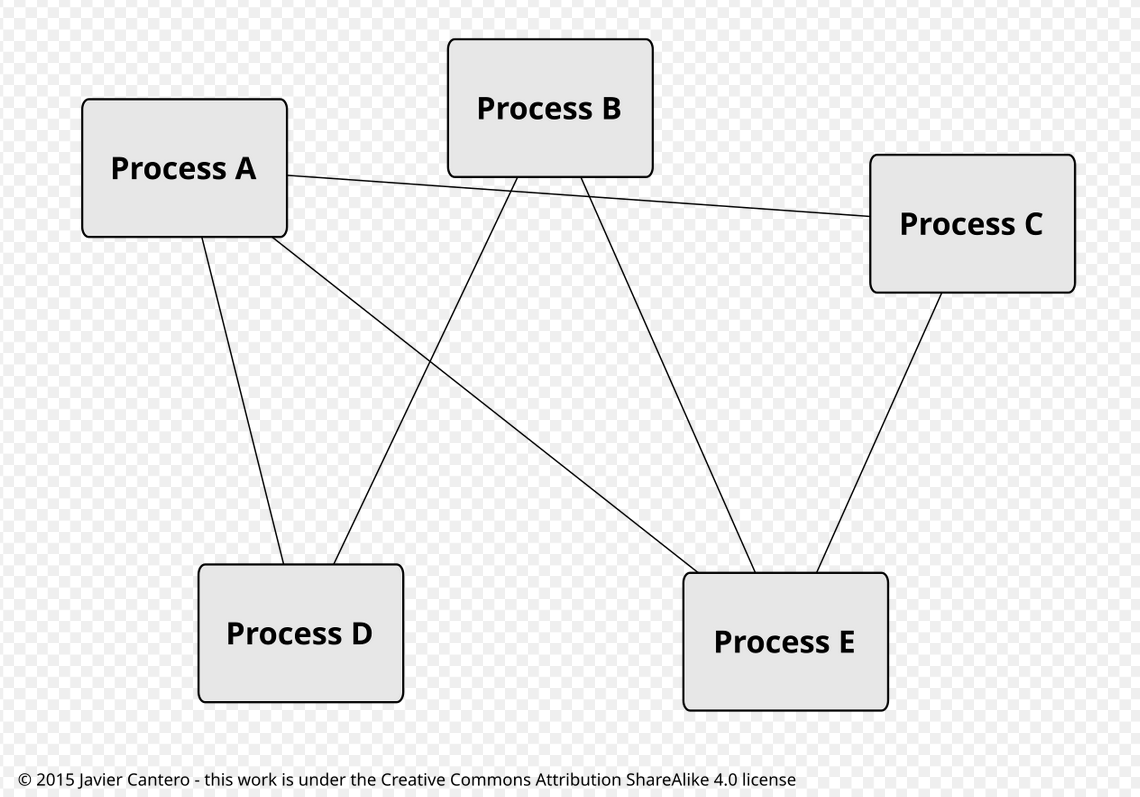
\includegraphics[width=\textwidth,height=\textheight,keepaspectratio]{ipc.png}
\end{frame}

\begin{frame}
    \frametitle{Przykłady}
        \begin{itemize}
        \item Pamięć współdzielona
        \item Sockety
        \item Pipe, named pipe
    \end{itemize}
\end{frame}

\begin{frame}
    \frametitle{Wysokopoziomowe rozwiązania}
    \begin{itemize}
        \item CORBA, Common Object Request Broker Architecture
        \begin{itemize}
            \item Skomplikowany, złożony standard
            \item Transparentność lokacji
            \item Kompatybilność
        \end{itemize}
        \item DCOP, Desktop COmmunication Protocol
        \begin{itemize}
            \item Część KDE...
            \item ...do czasu D-Busa, KDE 4
        \end{itemize}
    \end{itemize}

\end{frame}


\begin{frame}
    \frametitle{freedesktop.org}
    Projekt z 2002 roku zarządzający między innymi:
    \begin{itemize}
        \item PulseAudio
        \item systemd
        \item Wayland
        \item Mesa
    \end{itemize}

\end{frame}
    




\section{Teoria}
\begin{frame}
    \frametitle{D-Bus}
    Potrzeba zaimplementowania ustandaryzowanego,
    bezpiecznego IPC dla
    środowisk graficznych.

    2002 - początek projektu

    2006 - stabilna wersja
\end{frame}

\begin{frame}
    \frametitle{Działanie}
    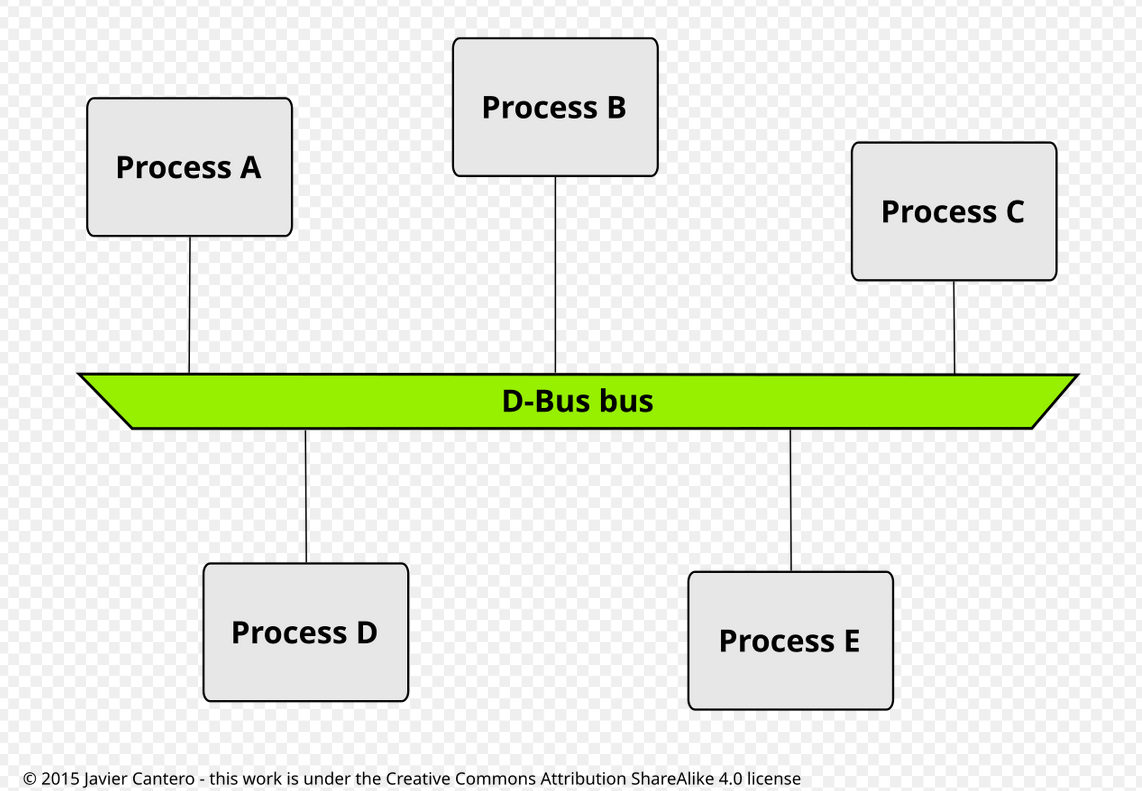
\includegraphics[width=\textwidth,height=\textheight,keepaspectratio]{dbus.png}
\end{frame}

\begin{frame}
    \frametitle{Zalety}
    \begin{itemize}
        \item Relatywnie prosty (ale nie libdbus...)
        \item Dostępność standardu w wielu językach programowania
        \item Security policy
        \item Abstrakcja połączenia
    \end{itemize}
\end{frame}

\begin{frame}
    \frametitle{D-Bus bus}
    Demon do którego łączą się aplikacje. Przekierowuje
    wiadomości od aplikacji do innych aplikacji. Zaimplementowany
    w libdbus.
\end{frame}

\begin{frame}
    \frametitle{libdbus}
    Niskopoziomowa biblioteka pozwalająca aplikacjom na wymianę 
    wiadomości.
\end{frame}

\begin{frame}
    \frametitle{System bus}
    Z poziomu użytkownika, osobna instancja dla każdego.
    \begin{itemize}
        \item GUI KDE, GNOME
        \item Aplikacje, Spotify, Firefox
        \item PulseAudio
    \end{itemize}
\end{frame}

\begin{frame}
    \frametitle{Session bus}
    Z poziomu systemu operacyjnego.
    \begin{itemize}
        \item Sieci, NetworkManager
        \item Urządzenia, UDisks, USB
        \item Uprawnienia, PolicyKit
    \end{itemize}
\end{frame}

\begin{frame}
    \frametitle{Połączenie serwisu}
    Następuje przy połączeniu do demona.
    Serwis ma przyznawaną nazwę:
    \begin{itemize}
        \item Unikalna: :1-37, :1-42
        \item Well-known name: org.Cinammon, org.mpris.MediaPlayer2.spotify
        \item Znak : zarezerwowany
    \end{itemize}
\end{frame}

\begin{frame}
    \frametitle{Obiekt}
    \begin{itemize}
        \item Wymaga określenia bus name
        \item Ścieżka do obiektu jako nazwa: 
        \begin{itemize}
            \item /org/Cinnamon 
            \item /com/Test
            \item /org/kde/kspread/sheets/3/cells/4/5
        \end{itemize}
        \item Implementuje interfejsy
        \item Implementuje sygnały i metody
    \end{itemize}
\end{frame}


\begin{frame}
    \frametitle{Interfejsy}
    Zbiór metod, sygnałów oraz właściwości (properties).
    Implementowane przez obiekty. 
    Coś jak abstract class.
\end{frame}

\begin{frame}
    \frametitle{Przykład}
    \begin{columns}
    \begin{column}{0.5\textwidth}
        \begin{center}
            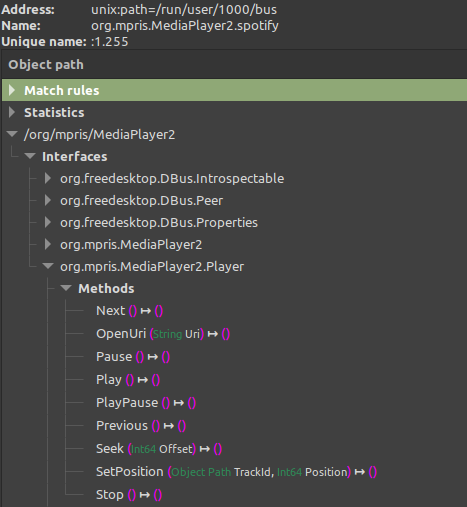
\includegraphics[width=\textwidth,height=\textheight,keepaspectratio]{service1.png}
        \end{center}
    \end{column}
    \begin{column}{0.5\textwidth}
        \begin{center}
            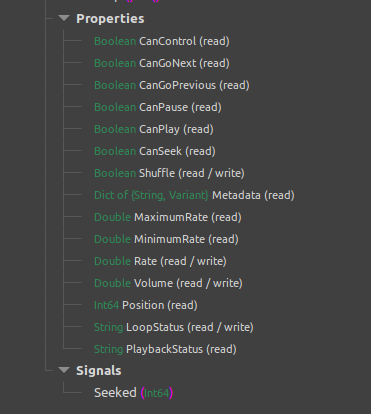
\includegraphics[width=\textwidth,height=\textheight, keepaspectratio]{example2.png}        
        \end{center}
    \end{column}
\end{columns}
\end{frame}


\begin{frame}
    \frametitle{System typów}
    \href{https://dbus.freedesktop.org/doc/dbus-specification.html}{Parę przykładów:}
    \begin{itemize}
        \item aai - tablica tablic intów
        \item a(ss) - array structów z dwoma stringami
        \item a\{sd\} - mapa klucz-string value-double
        \item v - variant, dynamiczny typ
        \item a\{sv\} - mapa z wartościami o różnych typach
    \end{itemize}
\end{frame}





% https://dbus.freedesktop.org/doc/dbus-api-design.html

\section{Praktyka}




%\begin{frame}
%    \frametitle{Co możemy implementować?}
%    Istnieje wiele interfejsów z możliwością implementacji.
%    Przykładowe API do implementacji:
%    \begin{itemize}
%        \item Interfejsy standardowe
%        \item \href{https://specifications.freedesktop.org/mpris-spec/latest/}{Standard MPRIS}-odtwarzacze muzyki
%    \end{itemize}
%\end{frame}

\begin{frame}[fragile]
    \frametitle{XML}
    \lstset{
    basicstyle=\tiny\ttfamily, 
    breaklines=true,           
    breakatwhitespace=true,    
    stepnumber=1               
}
    \begin{lstlisting}
    <node>
        <interface name="org.meks.Logger">
            <method name="AddLog">
                <arg direction="in"  type="s" name="log_str" />
                <arg direction="out" type="s" />
            </method>
            <signal name="CountChange">
                <arg type="(ib)" name="count" />
            </signal>
            <property name="Upper" type="b" access="readwrite"/>
            <property name="LogCount" type="i" access="read" />
            <property name="LogFileName" type="s" access="readwrite"/>
        </interface>
    </node>

    \end{lstlisting}
\end{frame}


\begin{frame}
    \frametitle{Policy XML}
    Kontrola dostępu do serwisów, metod i sygnałów.
    Znajduje się w /etc/dbus-1/system.d lub /usr/share/dbus-1/system.d

    Przykład: NetworkManager.conf
\end{frame}



\begin{frame}
    \frametitle{Narzędzia}
    \begin{itemize}
        \item dbus-monitor - debugger do monitorowania wiadomości dbusa
        \item dbus-send - wysyłanie wiadomości do busy
        \item d-feet - graficzny debugger do sprawdzania
        serwisów i wysyłania wiadomości
        \item busctl - komenda do badania serwisów
        \item gdbus-codegen - generowanie kodu w C, biblioteka GDbus
    \end{itemize}
\end{frame}

\begin{frame}
    \frametitle{Implementacje, Bindingi}
    Freedesktop.org oferuje implementacje i bindingi protokołu w D-Bus. Najciekawsze:
    \begin{itemize}
        \item libdbus - niskopoziomowe API w C, nie polecane do pisania 
        prostych aplikacji
        \item GDbus - niezależna od libdbus implementacja d-bus w C
        \item pydbus - wysokopoziomowy wrapper w pythonie na podstawie GDbus
        \item zbus, DBus-Java i inne
    \end{itemize}
\end{frame}


\begin{frame}
    \frametitle{Podsumowanie}
    \begin{itemize}
        \item IPC służące do wykonywania metod 
        i nasłuchiwania sygnałów serwisów
        \item Serwisy składające się z obiektów implementujących interfejsy
        z definicjami sygnałów, metod i właściwości(properties)
        \item Dobre do wymiany pojedynczych wiadomości
        \item Słabe do wymiany dużych danych
        \item Walidacja typów i autoryzacja dzięki security policy
    \end{itemize}
\end{frame}




\begin{frame}
    \frametitle{Źródła}
    \begin{itemize}
        \item     \href{https://dbus.freedesktop.org/doc/dbus-tutorial.html}{https://dbus.freedesktop.org/doc/dbus-tutorial.html}
        \item     \href{https://dbus.freedesktop.org/doc/dbus-specification.html}{https://dbus.freedesktop.org/doc/dbus-specification.html}
        \item     \href{https://www.freedesktop.org/wiki/IntroductionToDBus/}{https://www.freedesktop.org/wiki/IntroductionToDBus}
        \item     \href{https://dbus.freedesktop.org/doc/dbus-python/}{https://dbus.freedesktop.org/doc/dbus-python}
        \item     \href{https://en.wikipedia.org/wiki/D-Bus}{https://en.wikipedia.org/wiki/D-Bus}
        \item     \href{https://news.ycombinator.com/item?id=8648437}{https://news.ycombinator.com/item?id=8648437}
    \end{itemize}
\end{frame}


\end{document}